\documentclass[letterpaper,oneside]{scrartcl}
\usepackage{fullpage}
\usepackage[utf8]{inputenc}
\usepackage[pdftex]{graphicx}
\usepackage{tikz}
\DeclareGraphicsExtensions{.png,.pdf}
\graphicspath{{plots/}}
\usepackage{hyperref}
\usepackage{url}
\usepackage[round,sectionbib]{natbib}
\bibliographystyle{abbrvnat}
\usepackage[small]{caption}
\usepackage[small]{titlesec}
\renewcommand\familydefault{bch}

\definecolor{female}{HTML}{EF8A62}
\definecolor{male}{HTML}{67A9CF}
\definecolor{not-too-happy}{HTML}{FC8D59}
\definecolor{pretty-happy}{HTML}{FFFFBF}
\definecolor{very-happy}{HTML}{91CF60}
\definecolor{grey30}{HTML}{4D4D4D}
\newcommand{\key}[1]
  {\protect \tikz{\fill[#1] rectangle (1ex,1ex);}}

\title{Product graphics}
\author{Hadley Wickham and Heike Hofmann}
\begin{document}
\maketitle
  
\section{Introduction}

% JASA methods
% Infovis?

% Aims of this paper:
%
%  * emphasise the connection between area graphics and factorising 
%    probabilities
% 
%  * pull all area plots on a common footing - provide a grammar for 
%    categorical graphics

Area plots are the graphical equivalent of contingency tables, displaying how a total is broken down into components.  

display categorical data with a polygon, typically a rectangle, for each combination of the factors of interest, with the area proportional to the number of observations in that combination.  Because the total area for a graphic is usually constrained, an area plot serves to partition up this total, displaying proportions rather than counts.

Figure \ref{fig:cat-examples} illustrates some of these plots.

\begin{figure}[htbp]
  \begin{center}
  %  \includegraphics[scale=1]{file}
  \end{center}
  \caption{Area plot examples.}
  \label{fig:cat-examples}
\end{figure}

Hierarchical partitioning of space.

\section{Factorising}

Basic idea is factorising table of probabilities:

\begin{itemize}
  \item as products of marginal and conditional distributions
  \item as areas in plots
  \item as sums of parameters in log-linear models
\end{itemize}

Some notation: let capital letters refer to the sample space, and lower case particular values.

Let $f(x, y, z)$ be the 3d pmf function. We can can write this pmf as product of marginals and conditionals in many different ways.  We can decompose product graphics in a similar way.

\begin{itemize}
  \item $f(x, y, z) = f(x, y | z) f(z)$
  \item $f(x, y, z) = f(x | y, z) f(y, z)$
  \item $f(x, y, z) = f(x | y, z) f(y | z) f(z)$
\end{itemize}

It can be useful to display partial decompositions, i.e. just $f(x, y | z)$, which is still a 3 variable pmf, and is defined as 

\[ f(x, y | z) = \frac{f(x, y, z)}{\sum_{x = a, y = b} f(a, b, z)} \]

so that each category of z sums to one, and for any fixed value of z, $f(x, y | z)$ is a valid pmf.

\[ \forall b \sum_a f(a | b) = 1 \]

Because of their hierarchical nature, an area plot of $f(x, y, z)$ also shows $f(y, z)$ and $f(z)$.  

Based on the modelling specification of \citet{wilkinson:1973} we define an algebra for describing these tables.  

\begin{itemize}
  \item \verb|~ a| represents $f(a)$,
  \item \verb|~ a + b| represents $f(a, b)$
  \item \verb!~ a | b! represents $f(a | b)$
  \item \verb!~ . | a! is a special case of $f(a) = \frac{1}{\#A}$. 
\end{itemize}

By convention we will write the top most level of the product plot on the left, and lower levels to the right.  While $f(x, y, z)$ and $f(z, y, x)$ display the same counts, their interpretation is different because of which marginal tables you see.

Figure~\ref{fig:fact-simple} illustrates these ideas with the distribution of happiness and sex. We start with a plot where area broken down by happiness. We can then continue to factor this plot to also display sex - the area of each rectangle is proportional to the number of people who are happy with that sex, and the construction allows us to see the conditional distribution of sex within happy. In this case the breaks line up, suggesting that there is no difference in sex, given happiness.  This could be followed up by a formula hypothesis test.

Removing the marginal effect of happiness, as in the column on the far right, makes each of the top-level categories the same size, and makes it easier to compare the conditional distributions.  It's not that important in this case, but in the bar chart below, it allows us to see the conditional distribution, and in the case when there are many levels with very different probabilities it can make the plot much easier to read.

\begin{figure}[htbp]
  \centering
  \includegraphics[width=0.33\linewidth]{fact-happy}%
  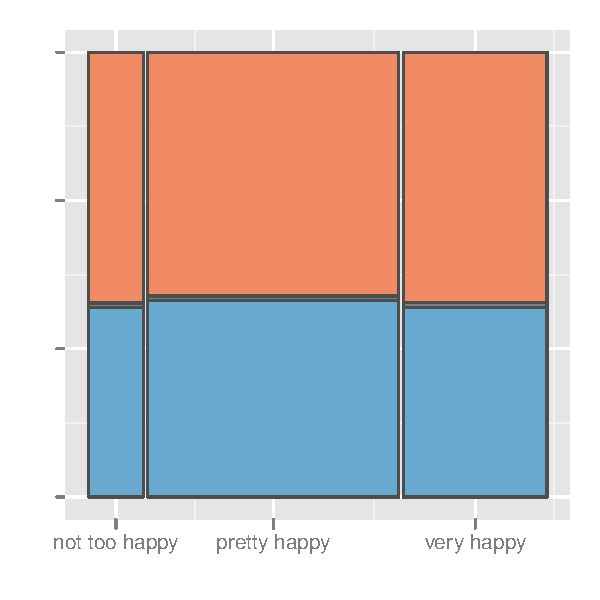
\includegraphics[width=0.33\linewidth]{fact-happy-sex}%
  \includegraphics[width=0.33\linewidth]{fact-happy|sex}

  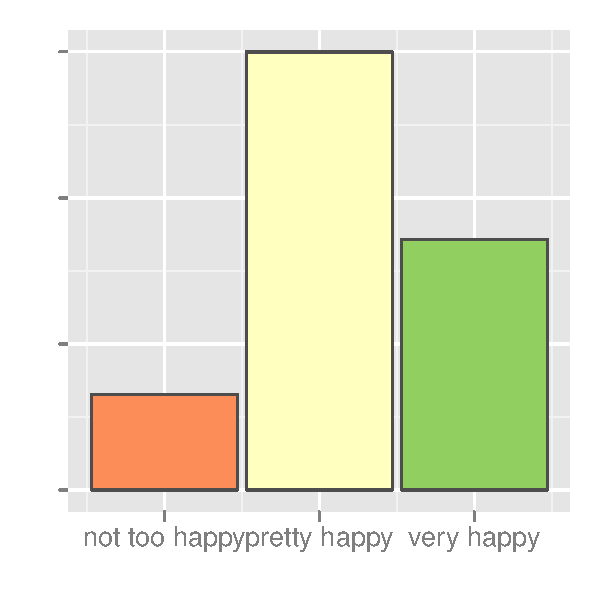
\includegraphics[width=0.33\linewidth]{fact-happy-2}%
  \includegraphics[width=0.33\linewidth]{fact-happy-sex-2}%
  \includegraphics[width=0.33\linewidth]{fact-happy|sex-2}

  \caption{Plots of the distribution of happiness and sex (\key{male} male, \key{female} female).}
  \label{fig:fact-simple}
\end{figure}


These techniques are also closely related to dimensional stacking \citep{leblanc:1990}

% Other papers to cite:
% 
% Generalised treemaps: \citep{vliegen:2006}
% Cocktailmaps: \citep{ahlberg:1996}
% Extension to mosaic: \citep{friendly:1999,hofmann:2000}
% Connection to models: \citep{theus:1999,hofmann:2001}


% Hierarchical coordinate systems 
%
% What are the common components of all these plots, and how can be describe
% them in a succinct way that also allows us to describe what tasks each
% display is good for?  We propose that there is one key feature that makes
% these plots special.  That is there their coordinate system, which is
% hierarchical.  
%
% In most coordinate systems that we are used to, such as Cartesian or polar
% coordinates, are symmetric in the sense that you can locate a point by
% starting from either dimension.  For example, in Cartesian coordinates you
% can identify either the x- or y-coordinate first, and the other next.  This
% also implies a distance symmetry when projected onto 2D Euclidean geometry.
% When you vary one coordinate by a small amount (holding all others constant)
% points in the projective geometry will be close.
%
% Neither of these properties hold for hierarchical coordinate systems. 
%
% We will discuss hierachical coordinate systems in general, and then present
% a specific hierachical coordinate system which gives rise to the area plots
% described previously. 

\section{Data}
\label{sec:data}

Two ways of representing data:

\begin{itemize}
  \item Multi-dimensional contingency table
  \item Data frame, with column of counts
\end{itemize}

The two are equivalent, but it's usually computational easier to work with the data frame version, because variables are explicit, and mathematically easier to work with the multidimensional array because multiplication is nicely defined.  Also deals better with sparsity and is common input to modelling algorithms.

Define the conditioning operator which makes the distribution uniform.  

In this paper, we'll use a small sample from the general social survey ({\sc gss}) focussing on happiness. 51\,020 observations from cross-section survey given yearly from 1972 to 2006.

\begin{itemize}
  \item Happy.  Discrete: ``very happy'', ``pretty happy'', ``not too happy''
  \item Age (in years), 18--89.
  \item Sex: ``female'', ``male''
  \item Degree: ``lt high school'', ``high school'', ``junior college'', ``bachelor'', ``gradudate''
  \item Relative financial status {\sf finrela}: ``far above average'', ``above average'', ``average'', ``below average'', ``far below average''
  \item Health: ``excellent'', ``good'', ``fair'', ``poor''
  \item Year: 1972--2006.
  \item Probability weight ({\sf wtsall}): 0.43--6.42.
\end{itemize}


\section{Display}
\label{sec:display}

Once we have made the decision to map area to proportion, we need to impose some constraints on the set of possible tilings of the plane. In general, we could also think of partitions of higher-dimensional spaces (e.g. 3d or 4d), but we will need to project these down to two for viewing anyway, so there is little disadvantage to working in 2d.

Some constraints are implied by our perceptual capabilities and others by geometry. On top of the constraint that area must be proportional to value, we add two additional constraints:

\begin{itemize}

  \item Partitions must be rectangular. It is easier to compare the areas of simple shape (i.e. rectangle vs polygon), and even better when one the length of one border is fixed, so we only need compare the length of the other \citep{cleveland:1984}. Rectangular partitions are also recursive in the sense that we can always tile a rectangle with smaller rectangles. This is not true for most shapes.

  \item Partitions must be disjoint. To be able to see the complete area of each rectangle they must be non-overlapping, and each split must be nested within the shapes of the previous level. Note that we do not impose the constraint that the tiling be space-filling. Space filling methods use will ensure that areas are larger, but make it harder to compare magnitudes because scales no longer align.

\end{itemize}

Note, however, that each of these constraints can be profitably relaxed. See Section~\ref{sec:relax} for details.

Let $a(i)$ give the area assigned to category $i$, which has proportion $f(i)$. Since we are using rectangles, $a(i) = k \dot a(i) = k \dot w(i) \times h(i)$ where $w$ and $h$ represent width and height respectively. Certain partitions also satisfy the constraint that $h(i) = \sqrt{k} f(i)^x$ and $w(i) = \sqrt{k} f(i)^y$ where $x + y = 1$. This is useful because it is only necessary to inspect one border to compare magnitudes.

The following two sections describe the partitions currently used to produce area graphics. Section~\ref{sub:part-1d} discusses partitions for 1d pmfs: bars, spines and tiles, Section~\ref{sub:part-2d} discusses one partition for 2d pmfs and Section~\ref{sub:part-nd} describes how the 1d and 2d primitives can be recursively combined to generate a partitioning for any higher dimension pmf and discusses how existing area graphics fall into this framework.

\subsection{1d primitives}
\label{sub:part-1d}

There are three 1d primitives, as shown in Figure~\ref{fig:part-1d}:

\begin{itemize}

  \item {\bf bar}s: height is proportional to value, width equally divides space. Bars allow comparison between absolute numbers, but are not space filling.  They occupy sum(values / max(values)) of the total area.  Bars can be arranged horizontally (``hbar'') or vertically (``vbar'').  Not space filling.

  \item {\bf spine}s: width is proportional to value, height equally divides space. Splines are space filling, but make it more difficult to compare absolute counts.  Splines can be arranged horizontally (``hspine''),  vertically (``vspine''), or can automatically pick their orientation (``spine'').  Space filling.

  \item {\bf tile}s: tile the plane with rectangles, trying to keep the aspect ratio of each rectangle close to 1. Comparing the areas is the most difficult perceptually, and are most useful when there are a large number of categories.  The is partitioning used by the squarified treemap \citep{bruls:1999}.  Not space filling.

\end{itemize}

\begin{figure}[htbp]
  \centering
    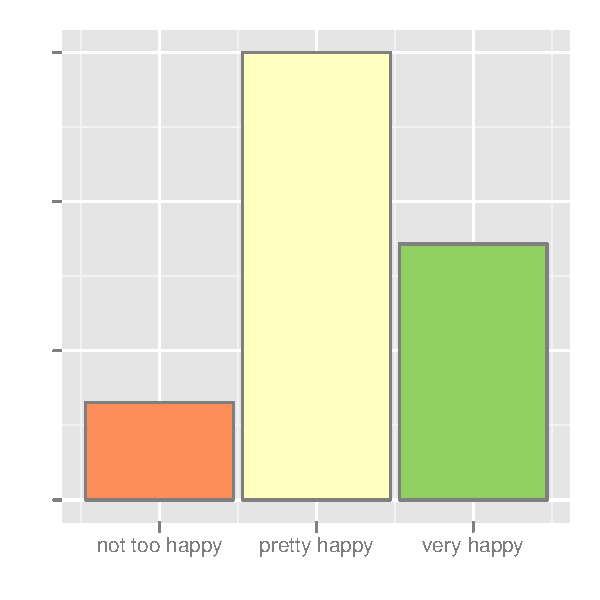
\includegraphics[width=0.33\linewidth]{part-hbar}%
    \includegraphics[width=0.33\linewidth]{part-hspine}%
    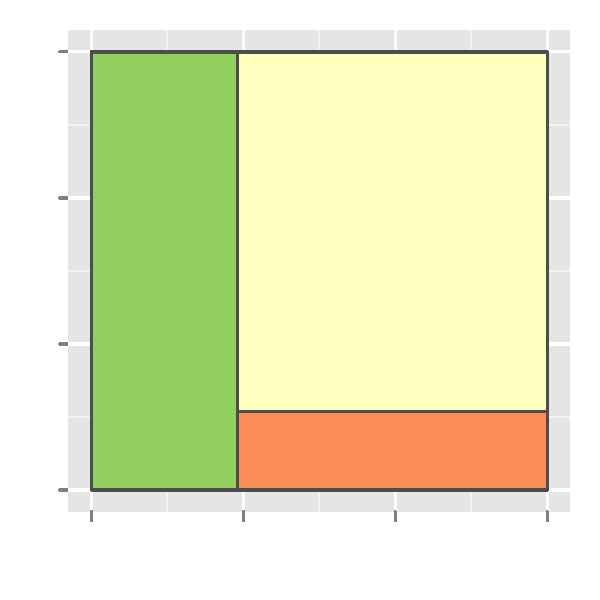
\includegraphics[width=0.33\linewidth]{part-treemap}

  \caption{1d partitions showing the distribution of happiness.  From left to right: bars, spines and tiles.}
  \label{fig:part-1d}
\end{figure}

The appearance of bars and splines is identical for uniformly distributed data.

\subsection{2d primitives}
\label{sub:part-2d}

We are currently aware of one 2d primitive, the {\bf fluct}: where width and height are proportional to the square root of the proportion. Flucts allow comparisons of relative magnitudes numbers in two directions. Each rectangle is arranged on a regular grid formed by the levels of the two variables, and thus the fluct is not space filling. A fluct displays a joint 2d distribution, unlike the combination of any two 1d partitions which display a conditional distribution.

One special case of the fluct is the equal bin size plot which occurs when the two variables are jointly uniformly distributed, usually as a result of conditioning. The equal bin size plot is useful to visualise missing combinations, or when supplemented with a third variable, to visualise the distribution conditional on two other variables.

\begin{figure}[htbp]
  \centering
    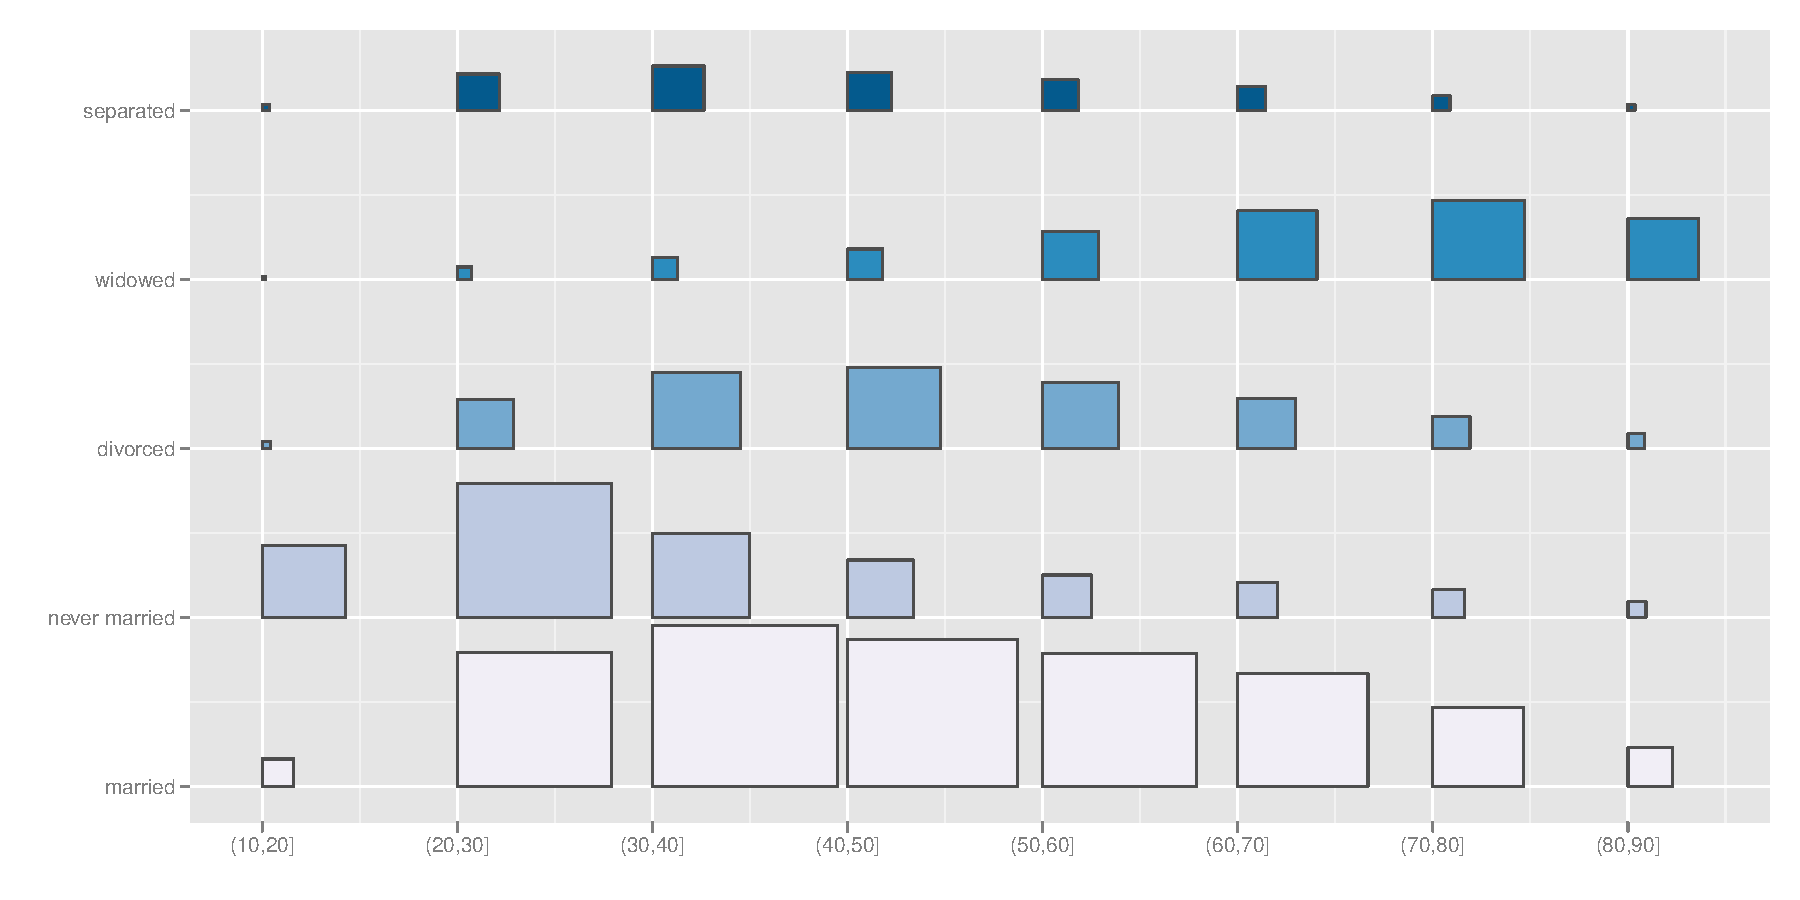
\includegraphics[width=0.5\linewidth]{part-fluct}%
    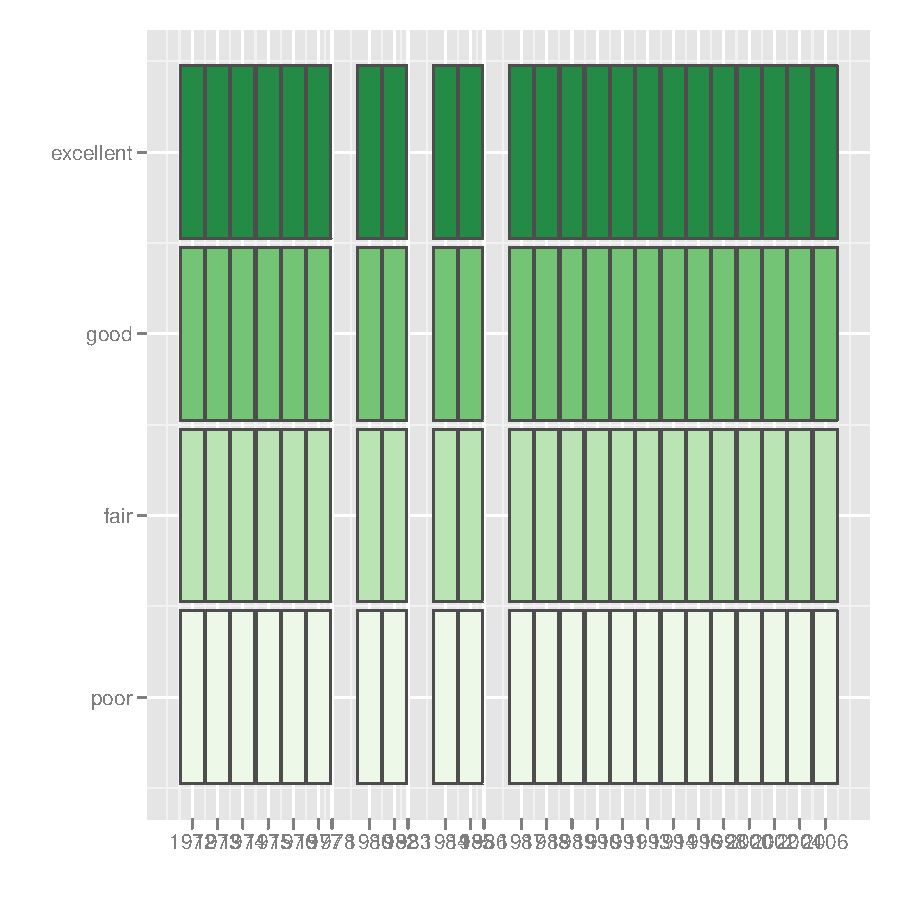
\includegraphics[width=0.5\linewidth]{part-fluct-cond}
  \caption{(Left) Distribution of age (in decades) and marital status.  All combinations of the two variables are present. (Right) Distribution of health status and year of survey. Health status was not recorded for three years.}
  \label{fig:fluct}
\end{figure}

\subsection{Combinations}
\label{sub:part-nd}

To visualise higher-dimensional pmfs, we recursively partition using the previously described primitives. That is, to display $f(x, y, z)$ we first create a partition based on $f(z)$ then partition each of those pieces based on $f(y | z)$ and again by $f(x | y, z)$. Figure \ref{fig:recursive} illustrates this process with a graphic that explores whether, conditional on marital status, there is a difference in happiness between men and women.  

% Heike: may be this would be a good spot for some of your Kronecker
% product theory?

\begin{figure}[htbp]
  \centering
    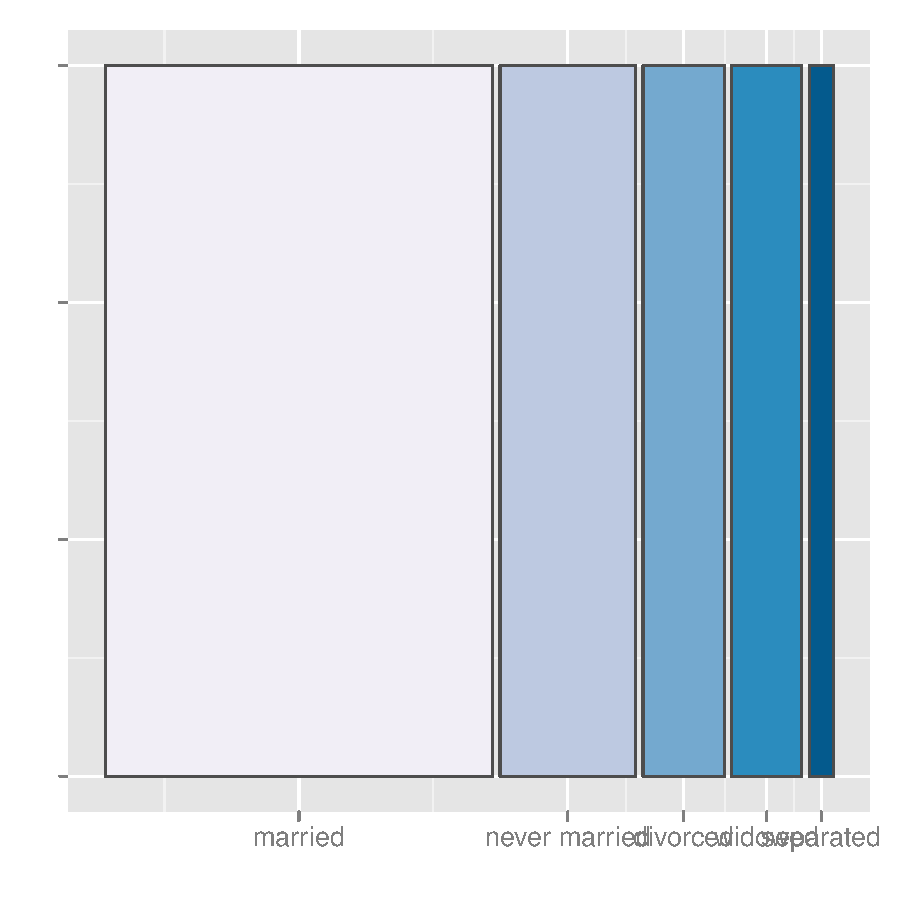
\includegraphics[width=0.33\linewidth]{part-comb-1}%
    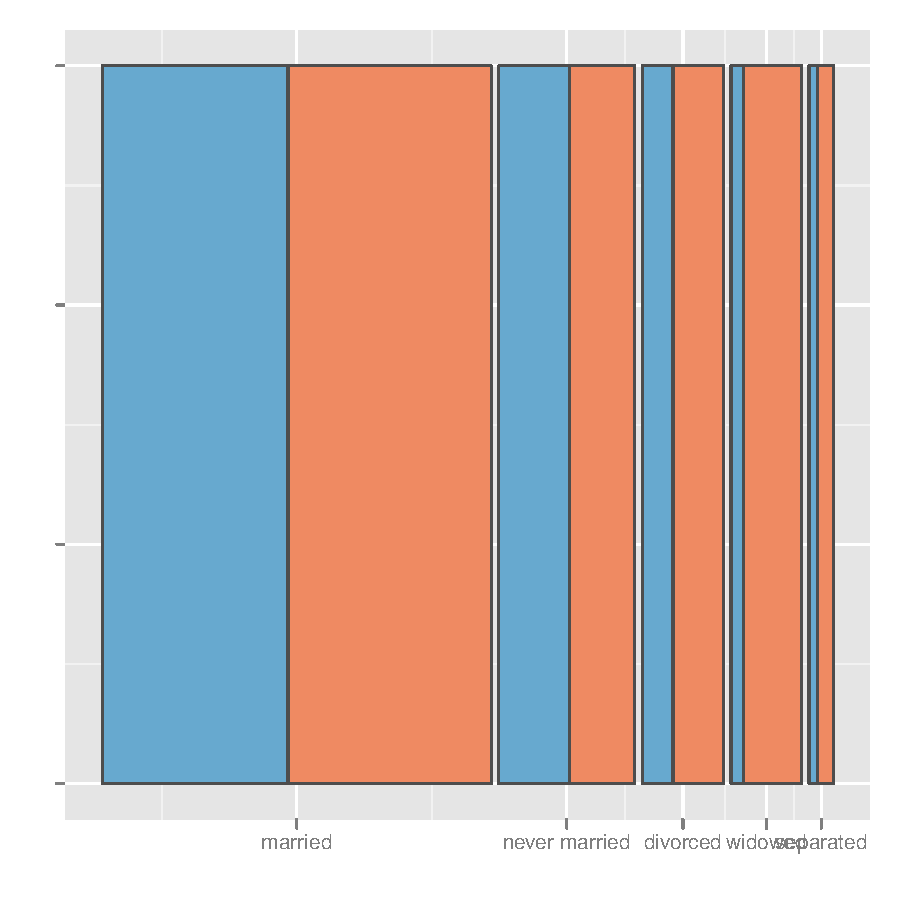
\includegraphics[width=0.33\linewidth]{part-comb-2}%
    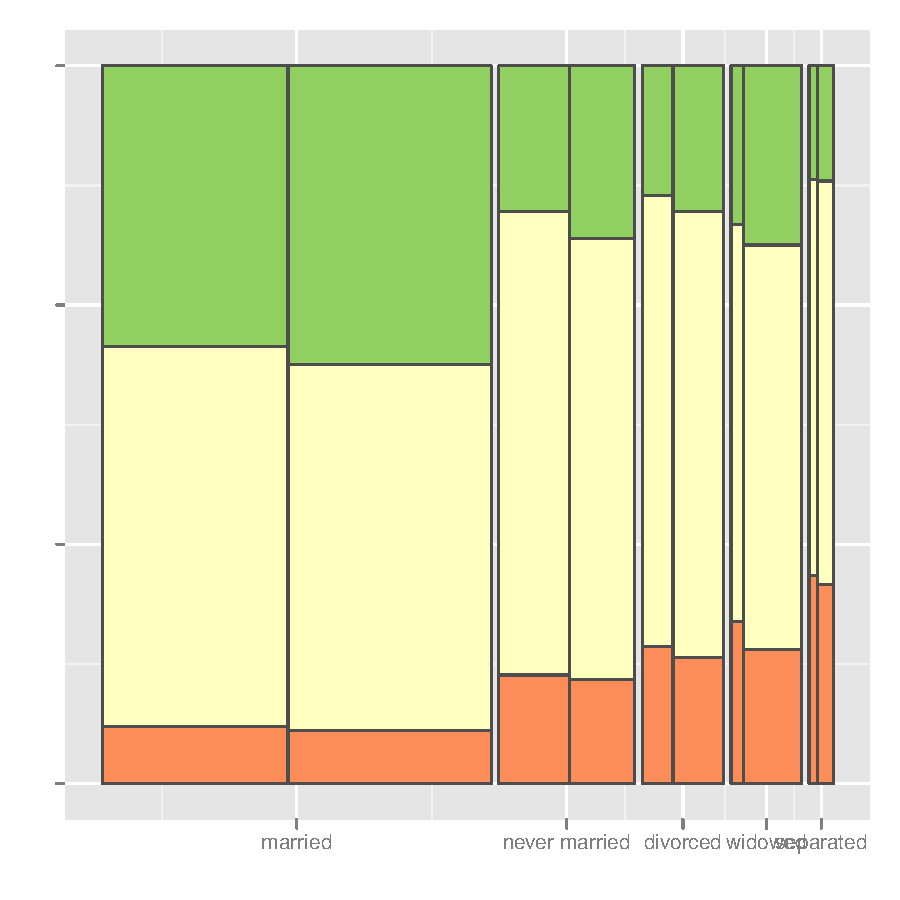
\includegraphics[width=0.33\linewidth]{part-comb-3}
  \caption{Conditional on marital status, are men or women happier?  This figure shows the construction of $\sim happy + sex + marital$ from (left to right) vspines by marital status, vspines by marital status and sex, and hspines by marital status, sex and happiness.  For all levels of marital status, men are slightly less happy.}
  \label{fig:recursive}
\end{figure}

The sequence of partitioning choices defines different named area plots:

\begin{itemize}
  \item {\bf Barchart} (1d). 1 hbar.
  \item {\bf Column chart} (1d). 1 vbar.
  \item {\bf Spineplot} (1d). 1 vspine.

  \item {\bf Stacked} barchart (2d). 1 hbar and 1 vspine.
  \item {\bf Nested} barchart (2d).  2 hbars. \citep{peltier:2009}
  \item {\bf Fluctuation} diagram (2d): fluct. 

  \item {\bf Equal bin size} plot (3d): fluct and vspine, provided the first two variables are uniform.

  \item {\bf Mosaic} plot (nd).  Alternating hspines and vspines.  \citep{hartigan:1984,hartigan:1981,friendly:1994,hofmann:2003}
  \item {\bf Double-decker} plot (nd).  $n-1$ hspines and 1 vspine. \citep{hofmann:2001}
  \item {\bf Treemap} (nd): n spines. \citep{shneiderman:1992}
  \item {\bf Squarified treemap} (nd): n tiles. \citep{bruls:1999}
  
\end{itemize}

Different combinations of partitions reveal different features of the data. Take for example, the distribution of age and marital status, as shown in Figure~\ref{fig:fluct}. Instead of visualisation the joint distribution with a fluct, we could focus on the conditional distribution of marital status, given age, or vice versa. Figure~\ref{fig:marital} shows two ways to do this. The left plot shows $\sim marital + age$ with a vspine nested in a hspine, and the right plot $\sim age + martial$ with a hbar nested in a vspine. These displays show the same data but are arranged in such a way to make different comparisons easier.

\begin{figure}[htbp]
  \centering
    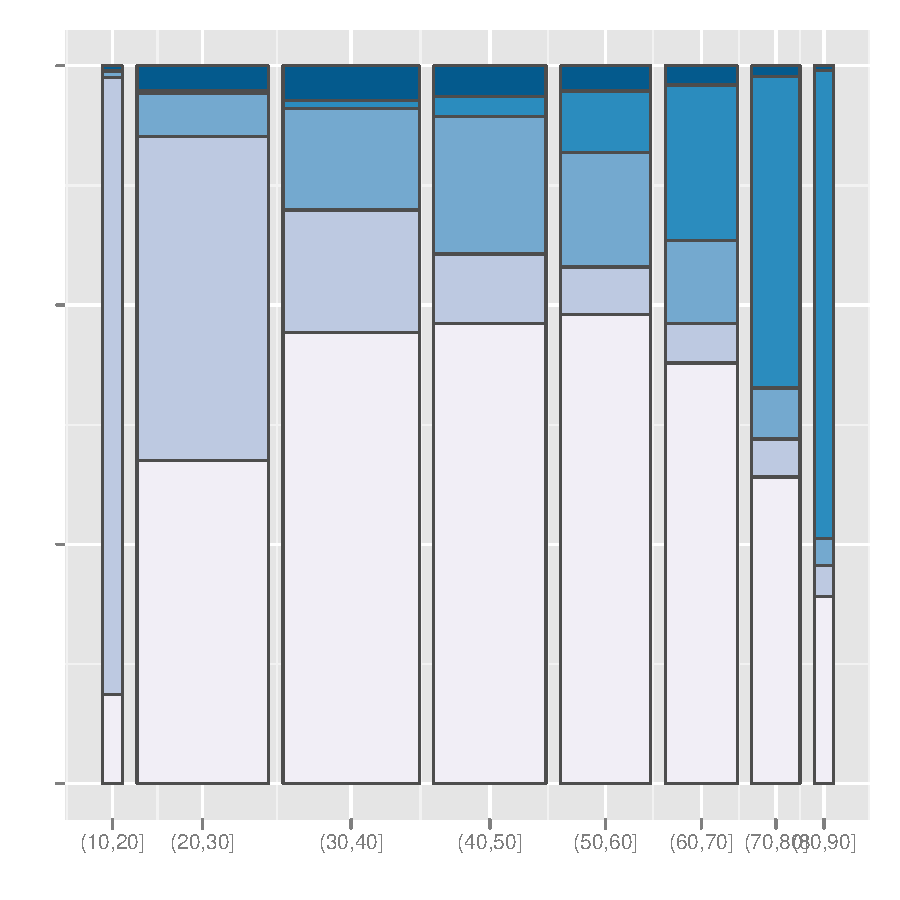
\includegraphics[width=0.5\linewidth]{part-marital-1}%
    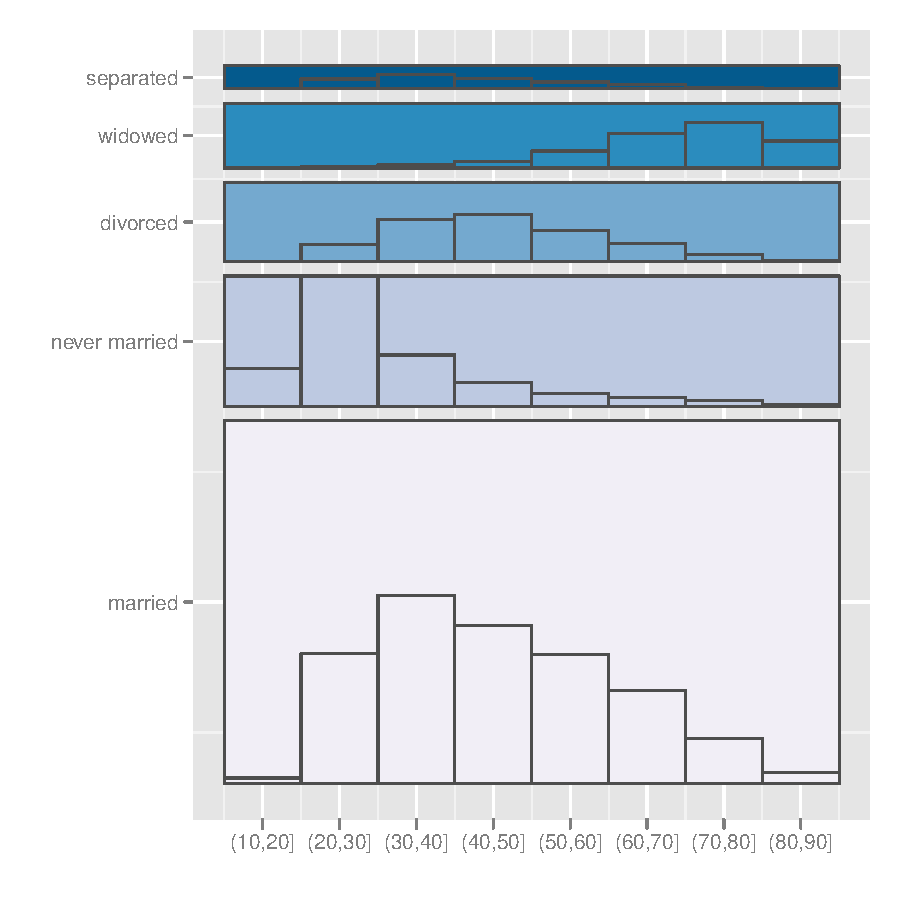
\includegraphics[width=0.5\linewidth]{part-marital-2}
  \caption{(Left) The joint distribution of marital status and age (in decades) partitioned by a vspine and hspine.  (Right) The joint distribution of age and marital status partitioned by a vspine and hbar.}
  \label{fig:marital}
\end{figure}

Conditioning is also an important tool, because it allows one to remove relationships that are well-known or uninteresting. Figure~\ref{fig:part-cond} uses a fluct and a vspine to explore the relationship between happiness, health and financial status. The left plot displays raw proportions, showing that most people are in good health and average financial standing. However, it is difficult to see how happiness varies within these conditions because the perceptual task is comparing areas. Conditioning on financial status and health produces the plot on the right (known as an equal bin size plot) and makes it easier to see the conditional distribution of happiness, because the perceptual task is simpler: comparing length on a common non-aligned scales.  Here we can see people tend to be happier the healthier and richer they are.

\begin{figure}[htbp]
  \centering
    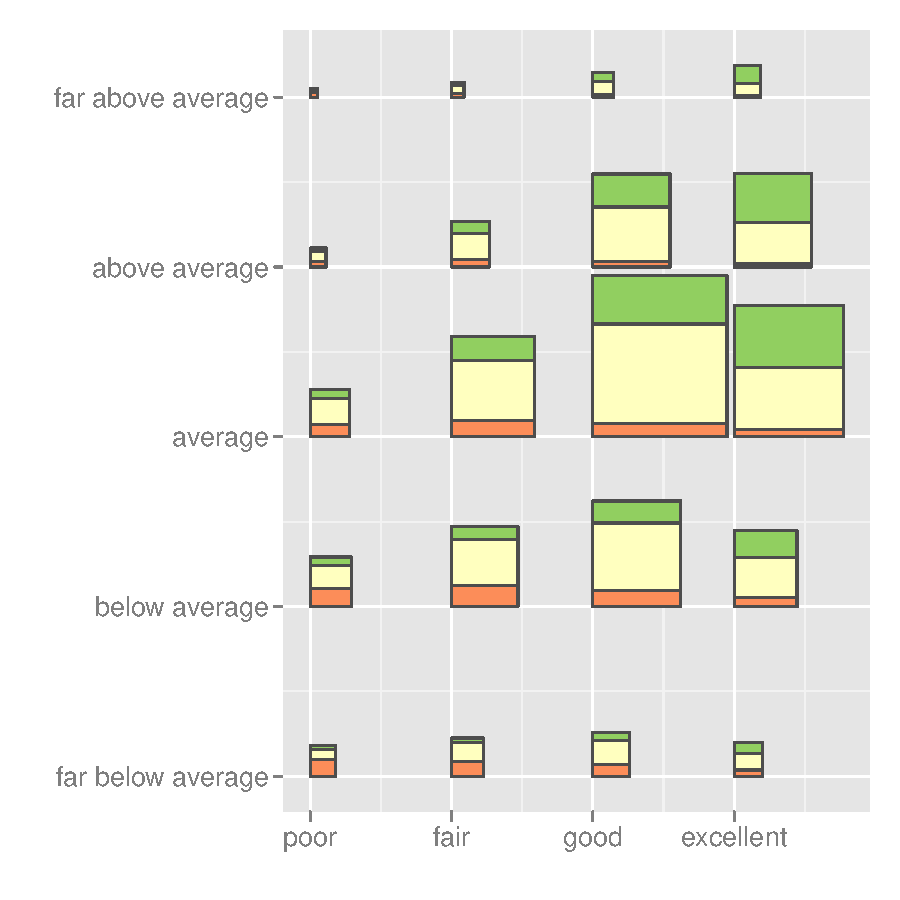
\includegraphics[width=0.5\linewidth]{part-fluctuation}%
    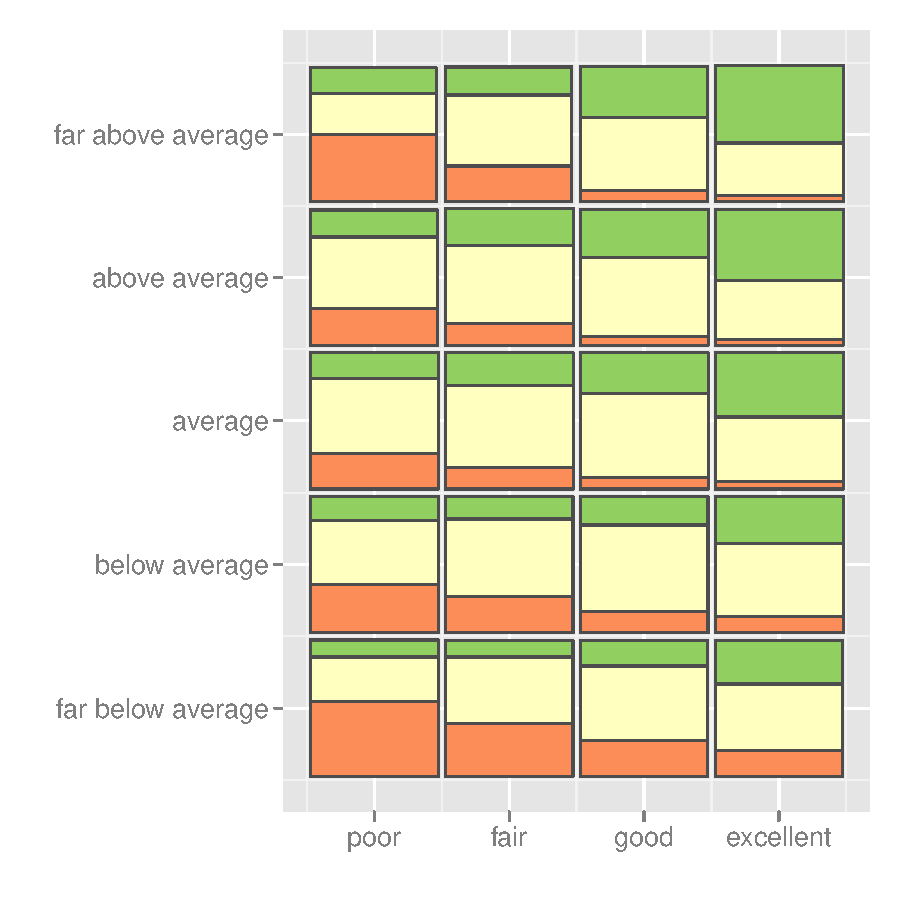
\includegraphics[width=0.5\linewidth]{part-equal-area}
  \caption{Two displays of $\sim happy + health + finrela$.  (Left) Unconditional values partitioned with a vspine and fluct.  (Right) Same partitions, but health and relative financial status conditioned to uniform distribution.  We can no longer see the joint distribution of health and financial status, but it is much easier to see the conditional distribution of happiness: healthier and richer people are happier. (Maybe money does buy happiness?).  (\key{not-too-happy} Not too happy, \key{pretty-happy} pretty happy, \key{very-happy} very happy)}
  \label{fig:part-cond}
\end{figure}

% http://peltiertech.com/Utility/ClusterStackUtility.html

Trellis graphics \citep{becker:1996}, as known as lattice or facetted or
conditioned graphics are another related display. They uses categorical
variables to generate multiple panels, each containing a plot of the subset of
the data. Trellised area plots also fall into our framework and can be
created by conditioning on the trellising variables.

\section{Relaxing constraints}
\label{sec:relax}

There are a number of cases in which it is useful to relax the constraints that we defined above.  These are described in sequence below.

\subsection{Area not proportional to weight}

It can be useful to violate the constraint that area should be proportional to weight to distinguish between zeros and very small values. A zero weight should have zero area, but giving it positive area can be useful, so you can actually see it! In general, it's useful to constrain all areas to be above a certain minimal perceptible size.  Areas which are constrained in such a way should have a visual flag (such as a difference colour) so ensure that the reader knows that the relationship between area and value has been violated.

On the other end of the spectrum, it can be useful to constrain put a cap on the largest possible values \citetext{Antony Unwin, priv. comm.}. By controlling this cap it is possible to zoom in on the smallest values.

Other non-linear transformations may also be useful.  For example, we could display the square root of the weights, to stabilise the variance of the areas.  If values span multiple orders of magnitude it may be useful to map log value to area.

\subsection{Non-disjoint partitions}

The cascaded treemaps of \citet{lu:2008} is an idea that illustrates how the violation of containment can be productive.  In the cascaded treemap, each level is slightly offset from the one above to create a pseudo-3d perspective.
This makes it easier to see all the levels of the hierarchy, not just the lowest level.  Figure~\ref{fig:cascade} shows an example of how cascading can help illuminate the structure of a complex mosaic plot.

\begin{figure}[htbp]
  \centering
    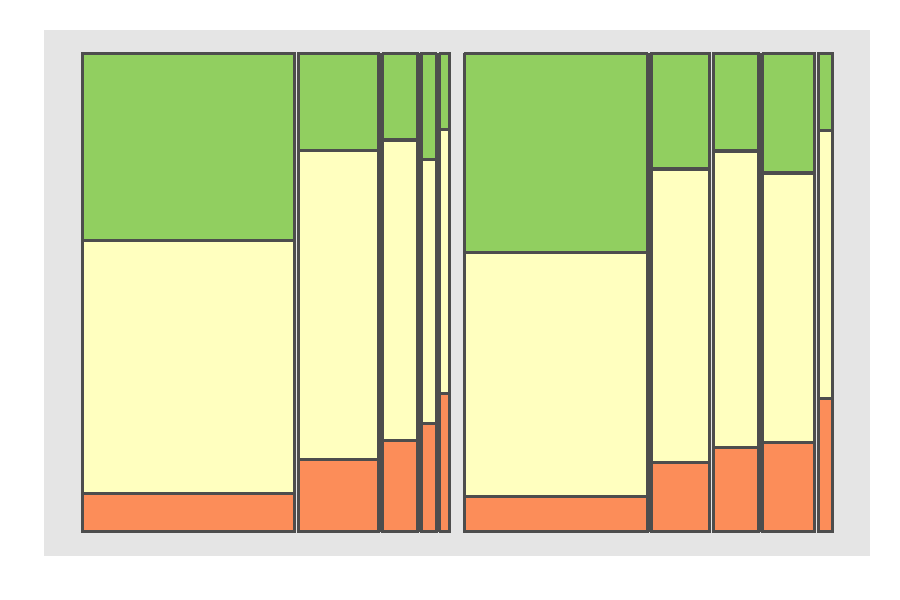
\includegraphics[width=0.5\linewidth]{sex-marital-happy}%
    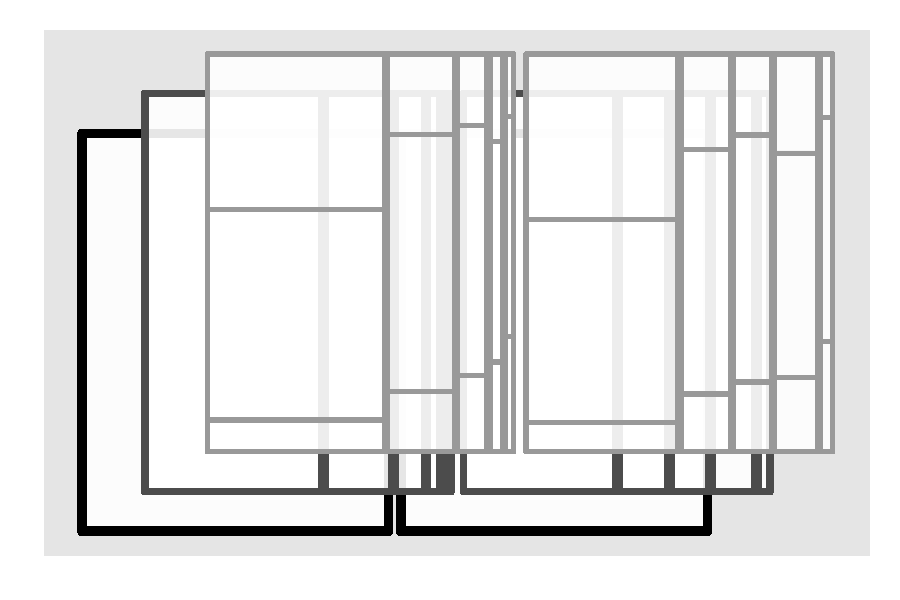
\includegraphics[width=0.5\linewidth]{cascade}
  \caption{A mosaic plot of happiness by martial status and sex. (Left) Coloured by happiness (\key{not-too-happy} Not too happy, \key{pretty-happy} pretty happy, \key{very-happy} very happy).  (Right) A cascaded view helps show how the plot is built up.}
  \label{fig:cascade}
\end{figure}

\subsection{Non-rectangular partitions}

A pie chart is a popular method of displaying proportions, but is not a rectangular partition. However, it turns out that there is a simple relationship between product plots and pie charts: an pie chart is an hspine drawn in polar coordinates with the x coordinate mapped to angle and the y coordinate to radius. Many other displays that use circular arcs turn out to be special cases of product plots, drawn in polar coordinates:   

\begin{itemize}
  \item Fourfold displays \citep{friendly:1995}, wind rose, sector graphic: hbar.

  \item Bullseye chart: hspine.

  \item Doughnut plot: vspine + hspine.

  \item Circular bar chart or racetrack plot: vbar.

  \item Infoslices \citep{andrews:1998}, nested vbar. But they only use half of the disk, and are specialised for highly nested data.

  \item Nightingales's coxcomb, is very similar to vspine / hbar in polar coordinates, except that the pie slices are overlapping and so violates the constraint of disjoint area.
\end{itemize}

\noindent Eight variants are displayed in Figure~\ref{fig:polar}.

To make this work more generally, the y-variable (mapped to radius) should be square-root transformed to ensure that that counts stay proportional to areas. The radial displays of \citet{stasko:2000} and fanlens of \citet{lou:2007} deliberately choose not to do this to highlight the outer levels.

\begin{figure}[htbp]
  \centering
    \includegraphics[width=0.25\linewidth]{hb-vb-cartesian}%
    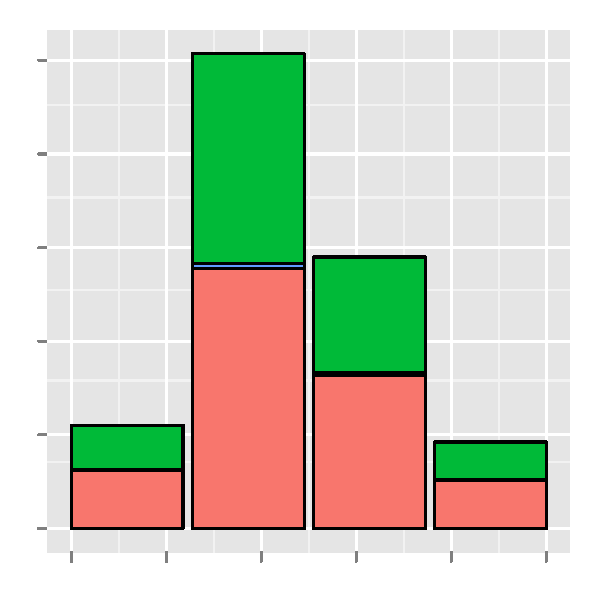
\includegraphics[width=0.25\linewidth]{hb-vs-cartesian}%
    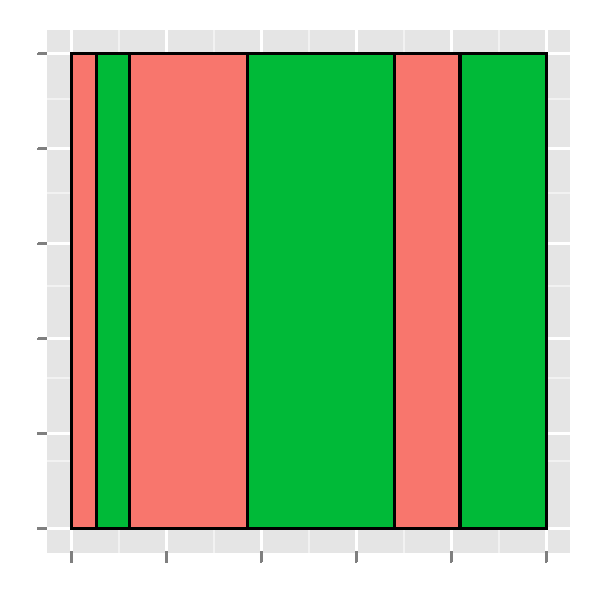
\includegraphics[width=0.25\linewidth]{hs-hs-cartesian}%
    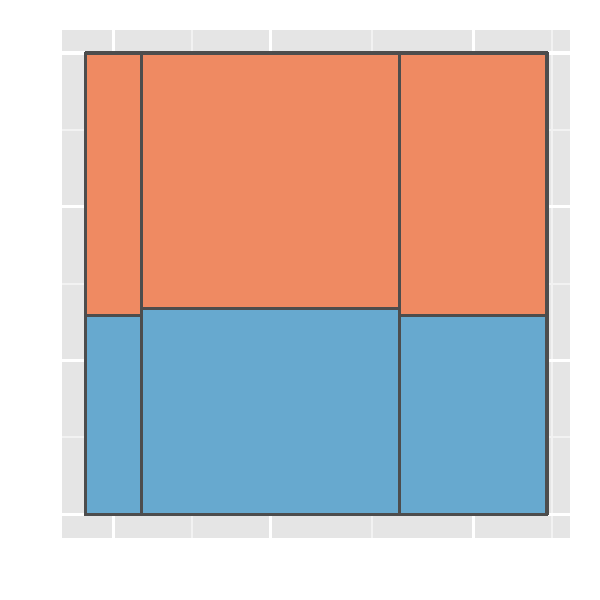
\includegraphics[width=0.25\linewidth]{hs-vs-cartesian}

    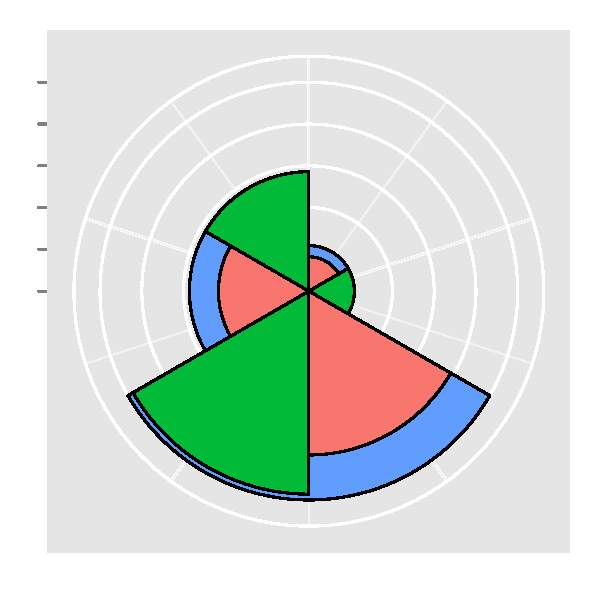
\includegraphics[width=0.25\linewidth]{hb-vb-polar}%
    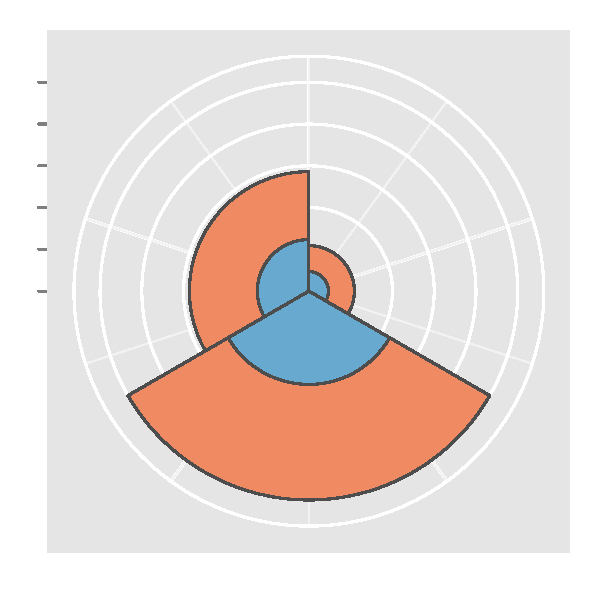
\includegraphics[width=0.25\linewidth]{hb-vs-polar}%
    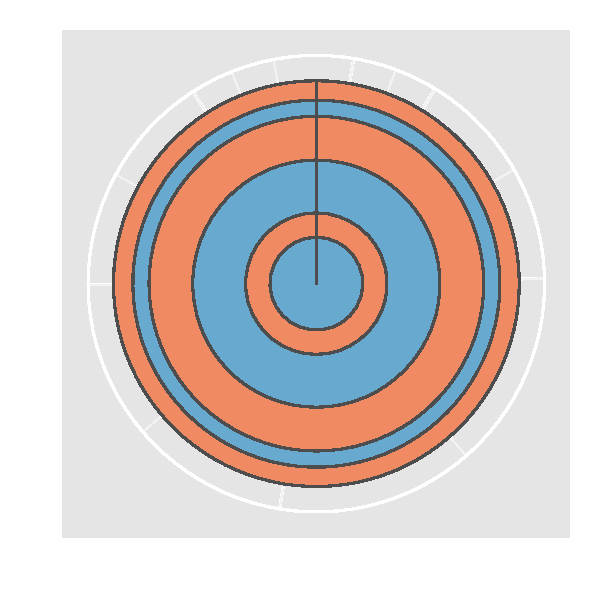
\includegraphics[width=0.25\linewidth]{hs-hs-polar}%
    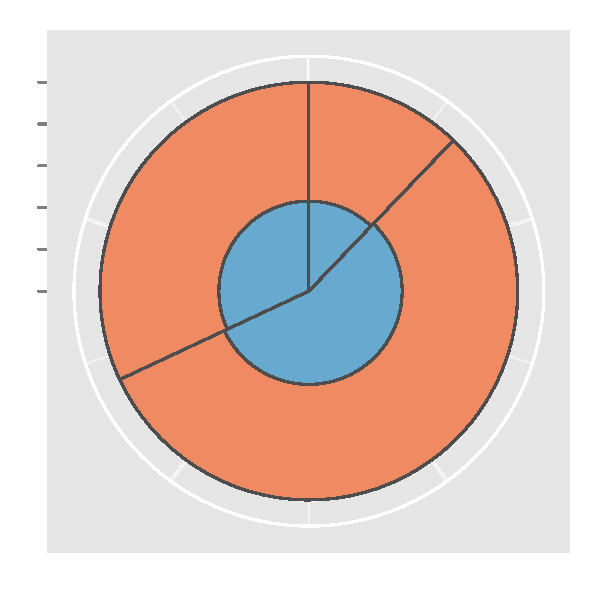
\includegraphics[width=0.25\linewidth]{hs-vs-polar}

    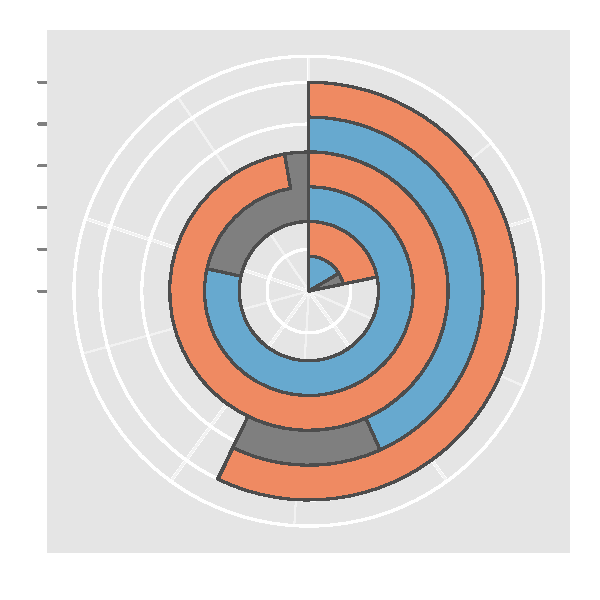
\includegraphics[width=0.25\linewidth]{hb-vb-polar-2}%
    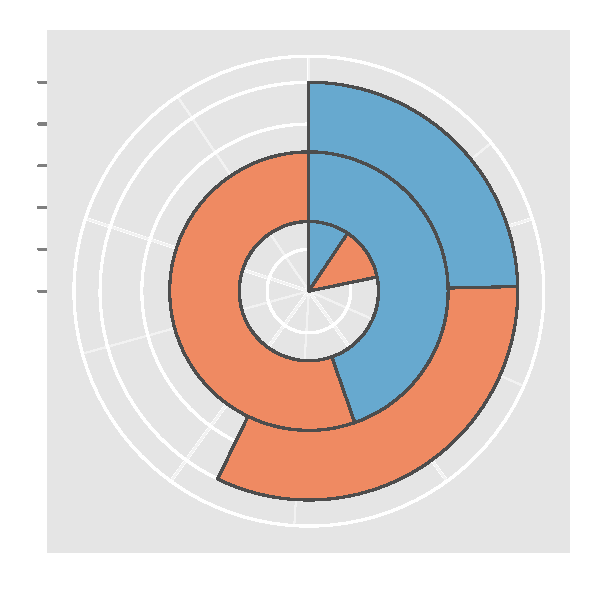
\includegraphics[width=0.25\linewidth]{hb-vs-polar-2}%
    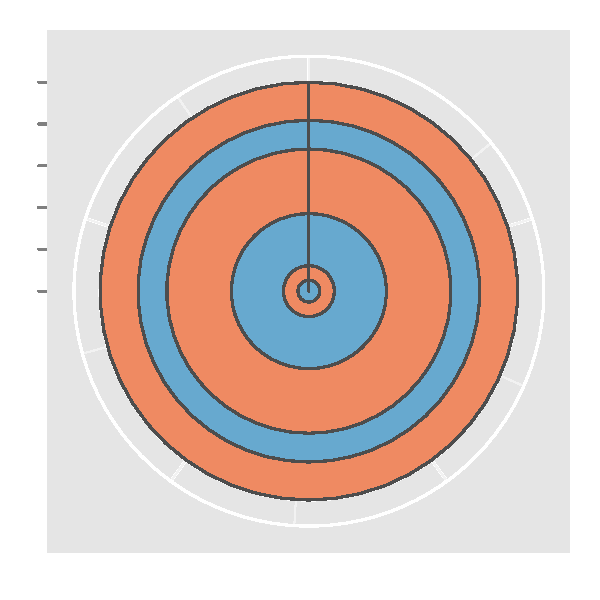
\includegraphics[width=0.25\linewidth]{hs-hs-polar-2}%
    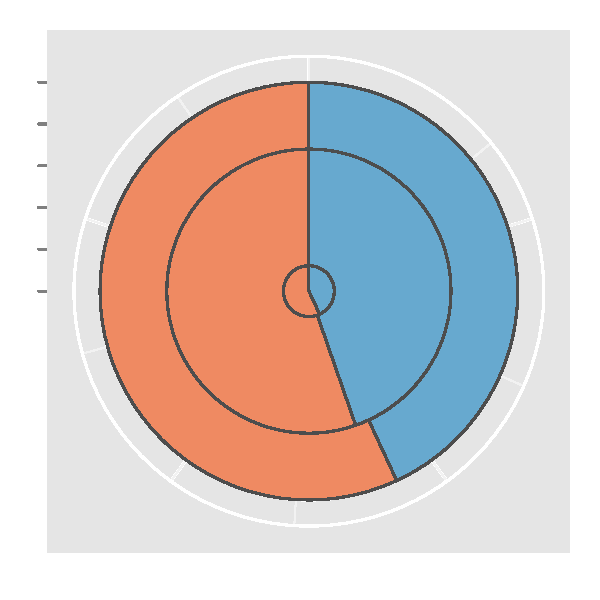
\includegraphics[width=0.25\linewidth]{hs-vs-polar-2}

  \caption{(Top) Area graphics in Cartesian coordinates. (Mid) Area graphics in polar coordinates. From left to right: hbar + hbar, vspline + hbar, hspine + hspine, hspine + vspine. (Bottom) Product graphics rotated 90 degrees before being converted to polar coordinates: vbar + vbar, hspline + vbar, vspine + vspine, vspine + hspine. (\key{male} male, \key{female} female)}

  \label{fig:polar}
\end{figure}

A number of non-rectangular treemaps have been proposed, such as the circular treemaps of \citet{wetzel:2008}, the space-filling curves of \citet{wattenberg:2005} and the voronoi treemaps of \citet{balzer:2005}.  However, because it is so much more difficult to compare the areas of arbitrary polygons, these approaches tend to be attractive rather than useful.

\section{Variations}
\label{sec:variations}

On top of this basic framework, there are a few variations designed for dealing with special types of data: missing data, weighted data, and continuous data.  These variations are described below.

\subsection{Missing values}
\label{sub:missing_values}



\subsection{Weighting}
\label{sub:weighting}

We have assumed that the probabilities represent counts, but without loss of generality, we can use any set of non-negative, additive weights. For example, in the happy dataset, the {\sf wtssall} variable gives analytic survey weights. Figure~\ref{fig:weighting} shows the difference between the weighted and unweighted distributions of age and sex. The distribution is subtly different. \citep{unwin:2007} describes the applications of weighted plots in more detail.

To express that we are displaying weights, rather than counts, we extend the formula syntax by putting the weighting variable on the left-hand side: $wtssall \sim sex + age$ vs. $ \sim sex + age$.

\begin{figure}[htbp]
  \centering
    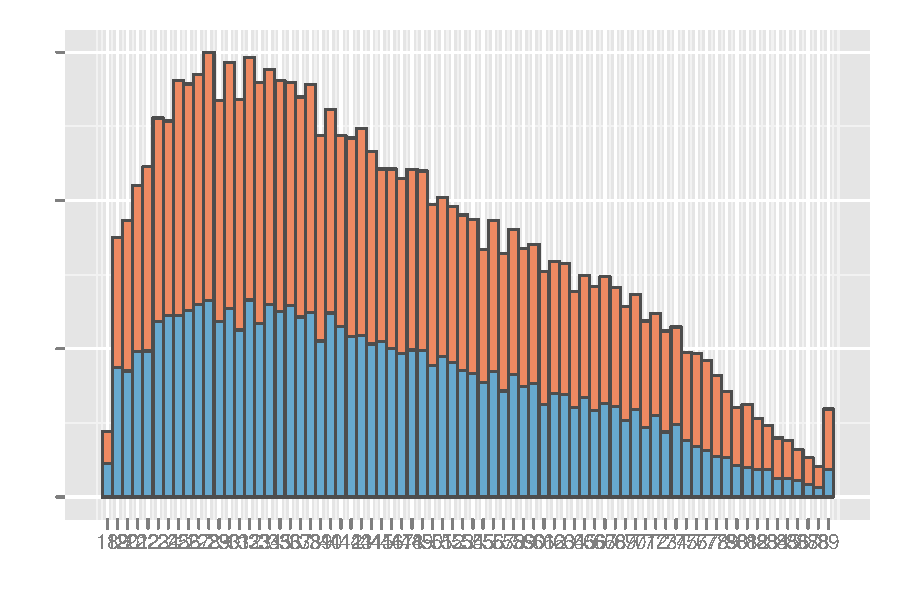
\includegraphics[width=0.5\linewidth]{wt-count}%
    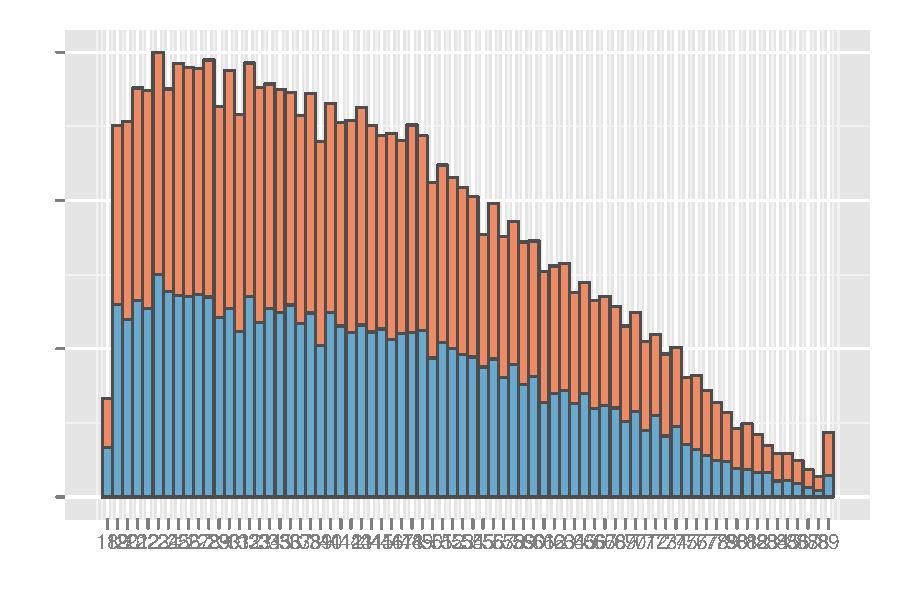
\includegraphics[width=0.5\linewidth]{wt-wtssall}%
  \caption{Joint distribution of age and sex (\key{male} male, \key{female} female). (Left) counts and (right) probability weights.}
  \label{fig:weighting}
\end{figure}

\subsection{Continuous data}
\label{sub:continuous_data}

These techniques can also be used with continuous data, if the data is binned to create a categorical variable. There are many different possible choices of binning algorithms, but we will focus on two:

\begin{itemize}
  \item Intervals of equal width.
  \item Intervals containing equal numbers of points.
\end{itemize}

This gives rise to the histogram and spinogram, analogues of the bar chart and spine chart respectively. A long standing tradition is that no gaps are displayed between adjacent rectangles when used for originally continuous data. Two examples are shown in Figure \ref{fig:cont-examples}.

\begin{figure}[htbp]
  \begin{center}
  \end{center}
  \caption{Area plots of originally continuous data}
  \label{fig:cont-examples}
\end{figure}

Give a few examples of non-traditional continuous-categorical plots.  Fluctuation diagram for exploring joint 2d distribution.  Mosaic for conditional.  Age and year distribution.  

Cat + continuous.

An alternative approach is use density estimates (or conditional density estimates) and plot with continuous area plots.  As in: Hofmann, H., Theus, M. (2005), Interactive graphics for visualizing conditional distributions, Unpublished Manuscript.

% \subsection{Nested data}
% \label{sub:nested_data}
% 
% Use space-filling!
% 
% We distinguish nested data from crossed data by the number of interactions with missing values.  Completely crossed data contains every combination of all variables.  Nested data contains 
% 
% 
% Aka sparse vs. dense.
% 
% It is not always possible to determine nested data from inspection of the data alone, but may need knowledge of the data collection.  For example, if a survey of teachers within schools was performed, and each teacher was identified by a identifier unique within a school, it might look like the data was only missing a few combinations, when in fact it is meaningless.  
% 
% 
% 
% Or when you have a hierarchy.
% 
% Example dataset - Doug Bates teachers/schools?
% 
% Possibilities: create new variable which is interaction of nested vars, or drop missings/zeros.  Treemaps deal almost exclusively with nested data.


\section{Labelling}
\label{sec:legends}

Due to the hierarchical nature of these plots, it's difficult to label them in an informative way. We take a pragmatic approach, and label a single horizontal and single vertical split, where possible, using colour to identify a third variable, if necessary. 

Understanding the composition of these plots is most easy when:

\begin{itemize}

  \item Exploration: You have interactive control over the creation of the plot, and can interactively query regions of interest
  
  \item Communication: The plot is built up step-by-step, and shows the minimum number of splits.  It may be easier to understand a single complex plot when factored into two or more simpler plots.

\end{itemize}

To create the labels in used in this paper, we inspect each level of the factorisation looking for the first level in which there are rows or columns.  We do this rather inspecting the partitions that make up the plot, because there are many possible combinations that create columns: hsplines, hbars, vsplines, vbars for uniform data, flucts, ... and then can occur at any level in the hierarchy depending on what's come before.

Apart from textual labels on the x-axis, other work has labelled individual cells with attributes of the data:

\begin{itemize}
  \item colour (map of the market)
  \item texture, such as in sieve plots \citep{friendly:2000}
  \item photographs \citep{bederson:2001}
  \item text (tables)
  \item embedded plots (time series in lab escape)
\end{itemize}

Or attributes of the hierarchy:

\begin{itemize}
  \item Spacing / borders
  \item Shading
  \item Cascading
  \item Labelling
\end{itemize}

\section{Conclusions} % (fold)
\label{sec:conclusions}

% section conclusions (end)

% bibtool -x product-graphics -o references.bib
\bibliography{references}
\end{document}
